\documentclass[paper=a4, fontsize=11.0pt, abstractoff, DIV12]{scrartcl}
\usepackage[utf8]{inputenc}
\usepackage[ngerman]{babel} % deutsche Rechtschreibung

\usepackage{graphicx} % Grafiken einbinden
\usepackage{amsmath} % AMS! Wichtig!
\usepackage{amsfonts} % mehr AMS
\usepackage{amssymb} % noch viel mehr
\usepackage[amssymb]{SIunits} % Einheiten anständig setzen
\usepackage{bbm} % fetter gedrucktes verfügbar machen, z.B. \mathbbm{1} = Eins mit Doppelstrich
\usepackage[Euler]{simpleMath}
\usepackage{tikz}
\usepackage{hyperref}
\hypersetup{colorlinks,
            breaklinks=true,
            linkcolor=black,
            urlcolor=black,
            citecolor=black,
            bookmarksnumbered,
            pdfauthor={Alexander Eberspächer},
            pdftitle={Übungen Theoretische Physik}}

\title{Mathematische Vorbereitungen zur Elektrodynamik}
\author{Alexander Eberspächer}
\date{\today}

\begin{document}
\maketitle
\begin{abstract}
Als Vorbereitung zur Vorlesung sollen kurz sowohl Ableitungen von
Vektorfeldern als auch vektorwertige Ableitungen besprochen werden. Die
Operationen Gradient, Rotation und Divergenz werden interpretiert und die
Integralsätze von Gauss, Stokes und Green werden kurz erläutert.
Ebenso wird an das Helmholtz-Theorem erinnert.\\[0.5ex]
Literatur: Arfken und Weber \cite{Arfken}.
\end{abstract}

\section{Gradient (und der \glqq Nabla\grqq-Operator)}

\subsection{Definition}

Betrachten wir eine Funktion $f = f(x,y)$ in zwei Dimensionen $x,y$. Die
Änderung $\dd f$ von $f$ zwischen $(x,y)$ und $(x+\dd x, y+\dd y)$ ist
\begin{equation}
\dd f(x,y) = f(x+\dd x, y+\dd y) - f(x,y)\, .
\label{eq:fDiff}
\end{equation}
Nach Taylor können wir nun für kleine $\dd x, \dd y$ den Ausruck $f(x+\dd x,
y+\dd y)$ um $(x,y)$ gemäß
\begin{equation*}
f(x+\dd x, y+\dd y) = f(x,y) + \firstpderiv{f}{x}\dd x + \firstpderiv{f}{y}\dd y
\end{equation*}
bis zur ersten Ordnung entwickeln. Setzen wir das in \eqref{eq:fDiff} ein,
so erhalten wir
\begin{equation}
\dd f(x,y) = \firstpderiv{f}{x}\dd x + \firstpderiv{f}{y}\dd y\, .
\end{equation}
Diesen Ausdruck können wir als Skalarprodukt der Vektoren
\begin{equation*}
\dd \vec r = \ZweierVec{\dd x}{\dd y}
\end{equation*}
und
\begin{equation*}
\nabla f := \ZweierVec{\partial_x f}{\partial_y f}
\end{equation*}
schreiben, es ist also
\begin{equation}
\dd f = \nabla f \cdot \dd \vec r \,.
\end{equation}
Den Vektoroperator
\begin{equation}
\nabla := \ZweierVec{\partial_x}{\partial_y}
\end{equation}
nennt man den \glqq Nabla\grqq-Operator.
Die Größe $\nabla f$ nennt man den Gradienten von $f$, man schreibt auch
$\grad f$ für $\nabla f$ . Die selben Begriffe
benutzt man gleichermaßen auch in drei Dimensionen. Eine alternative Schreibweise
für $\nabla$ ist dort natürlich
\begin{equation*}
\nabla = \vec{e}_x \firstpderiv{}{x} + \vec{e}_y \firstpderiv{}{y} + \vec{e}_z \firstpderiv{}{z}
\end{equation*}

\subsection{Geometrische Bedeutung des Gradienten}

Um die geometrische Bedeutung des Gradienten zu greifen betrachten wir eine
Fläche
\begin{equation}
f(x,y,z) = \const\, .
\label{eq:Flaeche}
\end{equation}
Die benachbarten Punkte $P, Q$ liegen auf dieser Fläche. Mit der (gerichteten) Entfernung $\dd \vec r$ gilt dann
\begin{equation}
\dd f = \nabla f \cdot \dd \vec r = 0\,.
\end{equation}
Weil $\dd \vec r$ im Allgemeinen ungleich $\vec 0$ ist, aber das Skalarprodukt
verschwindet, muss also $\nabla f$ \emph{senkrecht} auf der Fläche
\eqref{eq:Flaeche} stehen.

Eine weitere Aussage erhalten wir, wenn wir zwei benachbarte Flächen
$f(x,y,z) = C_1$ und $f(x,y,z) = C_2$ betrachten.

\begin{center}
    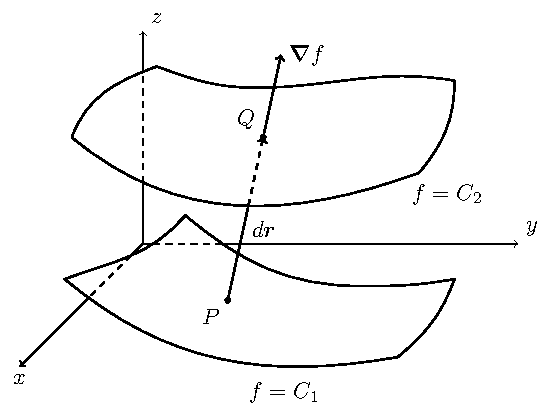
\includegraphics{Figures/Grad}
\end{center}
Hier ist
\begin{align}
\dd f = C_1 - C_2 = \Delta C &= (\nabla f)\cdot \dd \vec r\nonumber\\
&=\abs{\nabla f} \abs{\dd \vec r}\cos\left[\angle(\nabla f, \dd \vec r) \right]\,.
\end{align}
Wählen wir nun ein festes $\dd f$, so ist $\abs{\dd \vec r}$ minimal für den
Fall dass $\dd \vec r \parallel \nabla f$ ist, da in diesem Fall $\cos[\dots]=1$ gilt. Das bedeutet aber, dass $\nabla f$ in die \emph{Richtung des größten Anstiegs} von $f$ zeigt!

\section{Divergenz}

\subsection{Definition}

Betrachten wir eine (kompressible) Flüssigkeit, die mit der (lokalen)
Geschwindigkeit $\vec v= \vec v(\vec r)$ strömt und deren Dichte durch $\rho
= \rho(\vec r)$ gegeben ist. Das Produkt $\vec j = \rho \vec v$ nennen wir den Strom. Eine kleine Einheitenanalyse zeigt, dass
\begin{equation*}
[\vec j] = [\rho][\vec v] = \frac{\mathrm{kg}}{\mathrm{m^3}}\cdot\frac{\mathrm{m}}{\mathrm{s}} = \frac{\mathrm{kg}}{\mathrm{m^2}\cdot{s}}
\end{equation*}
die Einheit eines (Massen-) Flusses pro Zeiteinheit hat. Den Ausruck
\begin{equation}
\div \vec j = \nabla\cdot(\rho \vec v) = \firstpderiv{\left(\rho v_x\right)}{x} + \firstpderiv{\left(\rho v_y\right)}{y} + \firstpderiv{\left(\rho v_z\right)}{z}
\end{equation}
nennt man die Divergenz des Vektorfeldes $\vec j$.

\subsection{Bedeutung}

Um die Bedeutung der Divergenz zu verstehen betrachten wir ein Volumen $\dd V = \dd x \dd y \dd z$ an der Stelle $x=y=z=0$.

\begin{center}
    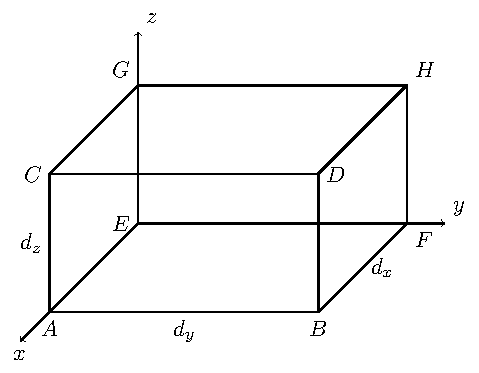
\includegraphics{Figures/Div}
\end{center}

Wir wollen nun den Fluß des Feldes $\vec j$ durch den Quader berechnen. Dazu
betrachten wir die Seitenflächen getrennt. In $x$-Richtung werden zwei
Flächen durchflossen. Durch diese strömt pro Zeiteinheit ein bestimmte Menge
Flüssigkeit:
\begin{itemize}
    \item Fläche $EFGH$, Fluß \glqq reinwärts\grqq: $\rho
    v_x\vert_{x=0}\, \dd y \dd z$
    \item Fläche $ABCD$, Fluß \glqq rauswärts\grqq: $\rho v_x\vert_{x=\dd
    x}\, \dd y \dd z$
\end{itemize}
Die Geschwindigkeitskomponenten $v_y$ und $v_z$ beschreiben einen Fluß
senkrecht zur betrachteten Fläche und tragen deswegen nichts bei. Den
zweiten Ausdruck entwickeln wir nach Taylor um $x=0$ bis zur ersten Ordnung,
es ist
\begin{equation*}
\rho v_x\vert_{x=\dd x} = \left[\rho v_x + \firstpderiv{(\rho v_x)}{x}\dd x\right]_{x=0}\, .
\end{equation*}
Damit lässt sich berechnen, wie viel Flüßigkeit netto in $x$-Richtung durch den
Quader strömt. Die Differenz der beiden Ausdrücke ist
\begin{equation}
\text{Netto-Fluss raus in \ensuremath{x}-Richtung} = \firstpderiv{\rho v_x}{x}\,\dd x\dd y\dd z\,.
\end{equation}
Die selbe Argumentation lässt sich mit den anderen Seiten des Quaders
wiederholen. Als Ergebnis findet man
\begin{align}
\text{Netto-Fluss pro Zeiteinheit rausw\"arts} &= \left[\firstpderiv{\rho v_x}{x} +  \firstpderiv{\rho v_y}{y} + \firstpderiv{\rho v_z}{z}\right]\, \dd x\dd y \dd z\nonumber\\
&=\nabla\cdot(\rho \vec v) \,\dd x\dd y\dd z\, .
\end{align}
Damit verstehen wir die Divergenz $\nabla \cdot \vec j$ direkt als
Netto-Fluß pro Zeiteinheit durch das Volumen $\dd x\dd y\dd z$.

Eine Anwendung ist die sogenannte Kontinuitätsgleichung
\begin{equation}
\firstpderiv{\rho}{t} + \nabla\cdot(\rho\vec v) = 0\,
\end{equation}
nach der eine Dichte-Änderung $\firstpderiv{\rho}{t}$ im Quader die direkte
Folge eines Netto-Flusses durch die Quaderoberfläche ist.

Im elektrostatischen Fall wird das elektrische Feld $\vec E$ von Relevanz
sein. Hier bedeutet dann $\nabla \cdot \vec E \ne 0$, dass sich im Quader
\emph{Quellen} oder \emph{Senken} des elektrisches Feldes befinden - diese sind
die definieren die Ladungsdichte (in SI-Eineiten) $\rho$ gemäß
\begin{equation}
\div \vec E = \frac{\rho}{\epsilon_0}\,.
\end{equation}

Das magnetische Feld $\vec V$ hingegen hat keine Quellen, da es keine
magnetische Ladungen gibt, es gilt also
\begin{equation}
\div \vec B = 0\,.
\end{equation}


\section{Rotation}

\subsection{Definition}

Unter der Rotation eines Vektorfeldes $\vec V$ verstehen wir
\begin{equation}
\rot \vec V = \nabla \times \vec V = \DreierVec{\partial_y V_z - \partial_z V_y}{\partial_zV_x - \partial_x V_z}{\partial_x V_y - \partial_y V_x}\,.
\label{eq:rotDef}
\end{equation}

\subsection{Anschauliche Bedeutung}

Der Strom einer Flüßigkeit sei durch eine Vektorfeld $\vec V$ beschrieben.
Wir betrachten die Zirkulation dieser Flüssigkeit in der $xy$-Ebene:

\begin{center}
    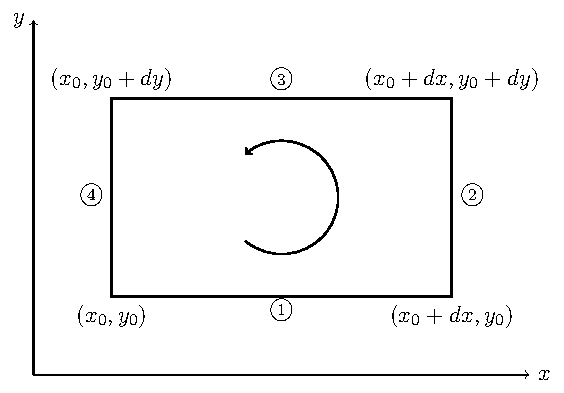
\includegraphics[width=0.6\textwidth]{Figures/Rot}
\end{center}

Das Linienintegral $\int \vec V \cdot \dd\vec\lambda$ über die Schleife zerlegen
wir dann in die Summe
\begin{align}
\text{Zirkulation\ensuremath{_{1234}}} = &\int\limits_{\circleText{1}} V_x \underbrace{\dd\lambda_x}_{=+\dd x} + \int\limits_{\circleText{2}} V_y \underbrace{\dd\lambda_y}_{=+\dd y}\nonumber\\
&+\int\limits_{\circleText{3}} V_x \underbrace{\dd\lambda_x}_{=-\dd x} + \int\limits_{\circleText{4}} V_y \underbrace{\dd\lambda_y}_{=-\dd y}
\end{align}
Wir beziehen nun alle Größen auf $(x_0, y_0)$ und entwickeln alle Ausdrücke nach
Taylor um diesen Punkt. Es ergibt sich
\begin{align}
\text{Zirkulation\ensuremath{_{1234}}} &= \underbrace{V_x(x_0, y_0)\dd x}_{\circleText{1}} + \underbrace{\left[V_y(x_0,y_0) + \firstpderiv{V_y}{x} \dd x  \right] \dd y}_{\circleText{2}}\nonumber\\
 &\quad+\underbrace{\left[V_x(x_0, y_0) + \firstpderiv{V_x}{y}\dd y\right](-\dd x)}_{\circleText{3}} + \underbrace{V_y(x_0, y_0)(-\dd y)}_{\circleText{4}}\nonumber\\
 &= \left(\firstpderiv{V_y}{x} - \firstpderiv{V_x}{y} \right)\,\dd x\dd y\,,
\end{align}
wobei alle partiellen Ableitungen an der Stelle $\vec r_0 = (x_0, y_0)$
ausgewertet werden. Die Korrekturterme stammen aus der Verschiebung der
Kanten $\circleText{3}$ und $\circleText{2}$ gegen die Kanten
$\circleText{1}$ und $\circleText{4}$. Durch Vergleich mit \eqref
{eq:rotDef} ist die Zirkulation des Feldes um die Schleife pro
Flächeneinheit dann also
\begin{equation}
\text{Zirkulation\ensuremath{_{1234}}}= \left(\nabla \times \vec V\right)_z\vert_{\vec r_0}\, .
\label{eq:Zirk}
\end{equation}
Analog lassen sich die anderen Koordinatenebenen behandeln.

Das führt zu einer sehr anschaulichen Definition der Rotation: positioniert
man einen kleinen Rotor in (frei drehbar, aber mit ortsfestem Schwerpunkt)
im Punkt $\vec r_0$ in der Flüssigkeit, so dreht sich der Rotor um diejenige
Achse, die durch $\nabla \times \vec V\vert_{\vec r_0}$ gegeben ist. Die
Rotationsgeschwindigkeit ist proportional zu $\abs{\nabla \times \vec
V}\vert_{\vec r_0}$.

Diese Diskussion findet sich etwas ausführlicher (und etwas
strenger/formaler) auch in \cite{Nolting}.

\section{Integralsätze}

Im Folgenden sollen ein paar sehr nützliche Integralsätze vorgestellt werden.

\subsection{Satz von Stokes}

Der Satz von Stokes lautet
\begin{equation}
\oint\limits_{\partial A} \vec V \cdot \dd \vec \lambda = \int\limits_{A} \left(\nabla\times\vec V\right)\cdot \dd \vec A\,.
\end{equation}
Demnach lässt sich der Fluß eines Rotationsfeldes $\nabla \times \vec V$
durch eine Fläche $A$ schreiben als ein Linienintegral entlang des Randes
$\partial A$ der Integrationsfläche.

\subsubsection{Anschauliche Interpretation}

Zerlege das Integrationsgebiet $A$ in viele kleine Rechtecke $\tilde A$:

\begin{center}
    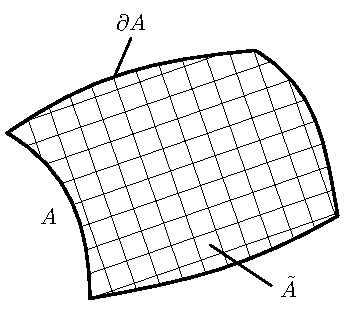
\includegraphics[width=0.4\textwidth]{Figures/Stokes1}
\end{center}
Für ein kleines Rechteck $\tilde A$ gilt nach \eqref{eq:Zirk}
\begin{equation*}
\sum\limits_{\text{4 Seiten}} \vec V \cdot \dd\vec\lambda = \left(\nabla\times\vec V\right)\cdot \dd \tilde{\vec{A}}\, .
\end{equation*}
Wenn man nun über alle kleinen Rechtecke summiert löschen sich Beiträge
benachbarter Rechtecke aus; da bei gleichem Umlaufsinn die Wegelemente
$\dd\vec\lambda$ entgegengerichtet sind.

\begin{center}
    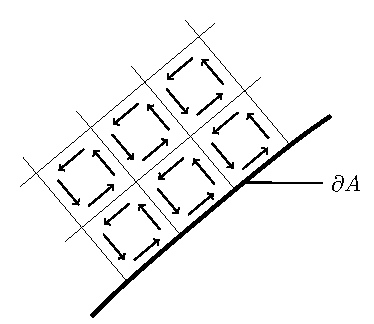
\includegraphics[width=0.4\textwidth]{Figures/Stokes2}
\end{center}
Es bleiben nur Beiträge vom Rand des Integrationsgebiets $A$! Damit gilt 
\begin{equation*}
\sum\limits_{\text{Rand von großer Fl.}} \vec V\cdot \dd \vec\lambda = \sum\limits_{\text{kleine Rechtecke}} \left(\nabla\times\vec V\right)\cdot \dd \tilde{\vec A}
\end{equation*}
Der Übergang zu infinitessmalen Größen führt dann auf den Satz von Stokes
\begin{equation*}
\oint\limits_{\partial A} \vec V \cdot \dd \vec \lambda = \int\limits_{A} \left(\nabla\times\vec V\right)\cdot \dd \vec A\,.
\end{equation*}
Eine wichtige Folgerung ergibt sich direkt aus diesem Satz: der Fluß eines
Wirbelfeldes $\nabla\times\vec V$ durch eine geschlossene Fläche $A$ (\emph
{kein} Rand) ist gleich $0$.

\subsubsection{Integraldarstellung der Rotation}

Der Satz von Stokes motiviert folgende Integraldarstellung der Rotation:

\begin{equation}
\left(\nabla \times \vec V\right)\cdot \vec n = \lim\limits_{A \to 0}  \oint\limits_{\partial A} \frac{\vec V \cdot \dd \vec \lambda}{\abs{A}} \,,
\end{equation}
wobei die Fläche $A$ eine Kreisscheibe ist, deren Fläche gegen $0$ strebt;
$\vec n$ steht normal auf der Kreisscheibe und $\dd \vec \lambda$ zeigt entlang
des Kreises.

\subsection{Satz von Gauss}

Laut dem Satz von Gauss gilt für den Fluß eines Feldes $\vec V$ durch eine
geschlossene Fläche $A = \partial V$
\begin{equation}
\oint\limits_{\partial V} \vec V \cdot \dd \vec A = \int\limits_{V} \nabla \cdot \vec V \dd V
\end{equation}

\subsubsection{Interpretation}

Zerlege das Integrationsvolumen $V$ in viele kleine Würfel. Es gilt dann für
einen Würfel
\begin{equation}
\sum\limits_{\text{6 Seitenfl.}} = \nabla\cdot\vec V \dd V\, .
\end{equation}

Summiert man nun über alle kleinen Würfel, so löschen sich bei benachabarten
innenliegenden Würfeln Flußbeiträge aus (Normalenvektoren \emph
{entgegengerichtet}!). Es bleiben nur die Beträge derjenigen Würfel, die am
Rande des Integrationsvolumen liegen.

\begin{center}
    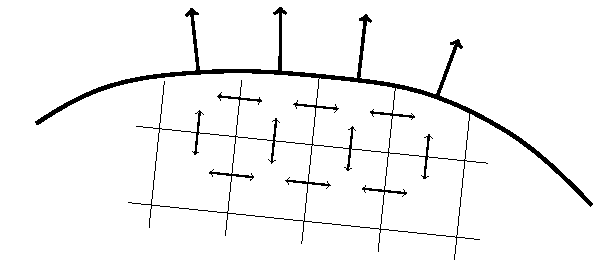
\includegraphics[width=0.5\textwidth]{Figures/Gauss}
\end{center}

Es gilt also
\begin{equation*}
\sum\limits_{\text{Aussenfl.}} \vec V \cdot \dd \vec A = \sum\limits_{\text{Würfel}}\nabla\cdot\vec V \dd V\, .
\end{equation*}
beziehungsweise im Übergang zu infinitessmalen Würfeln
\begin{equation}
\oint\limits_{\partial V} \vec V \cdot \dd \vec A = \int\limits_{V} \nabla \cdot \vec V \dd V\, .
\end{equation}


\subsubsection{Integraldarstellung der Divergenz}

Der Satz von Gauss motiviert die Integraldarstellung der Divergenz
\begin{equation}
\nabla\cdot \vec V = \lim\limits_{V\to P}\int\limits_{\partial V}\frac{\vec V \cdot \vec n}{\abs{V}}\,\dd A\,.
\end{equation}
In dieser Gleichung ist $V$ ein Integrationsvolumen, das den Punkt $P$
zusammengezogen wird; $A = \partial V$ ist der Rand von $V$, $\vec n$ ein
Normalenvektor auf $A$ und $\dd A$ ein (skalares) Flächenelement.

\subsection{Greensche Identitäten}

Aus dem Satz von Gauss lassen sich zwei weitere Identitäten folgern, die in der
Elektrodynamik gebraucht werden.

Zunächst benutzen wir die beiden Gleichungen
\begin{align}
\nabla\cdot\left(u\nabla v\right) &= u\Delta v + (\nabla u)\cdot(\nabla v)\label{eq:Green1}\\
\nabla\cdot\left(v\nabla u\right) &= v\Delta u + (\nabla v)\cdot(\nabla u)\label{eq:Green2}
\end{align}
für die skalare Funktionen $u$ und $v$. Beide Gleichungen folgen aus der
Produktregel. Wir ziehen nun \eqref{eq:Green2} von \eqref{eq:Green1} ab und
erhalten
\begin{equation*}
\nabla \cdot(u\nabla v) - \nabla\cdot(v\nabla u) = u\Delta v - v\Delta u\, .
\end{equation*}
Diese Gleichung integrieren wir über ein Volumen $V$ zu
\begin{equation*}
\int\limits_{V} \nabla\cdot \left[u\nabla v - v\nabla u\right]\,\dd V =\int\limits_{V} \left[ u\Delta v - v\Delta u\right]\,\dd V\, .
\end{equation*}
Wendet man den Gausschen Satz auf der rechten Seite (dort steht ein
Volumenintegral über eine Divergenz) an, so erhält man die erste Greensche
Identität
\begin{equation}
\oint\limits_{\partial V} \left[u\nabla v - v\nabla u\right]\cdot\dd \vec A = \int\limits_{V} \left[ u\Delta v - v\Delta u\right]\,\dd V\, .
\end{equation}

Die zweite Identität erhält man aus \eqref{eq:Green1} alleine.
Volumenintegration auf beiden Seiten führt auf
\begin{equation*}
\int\limits_{V}\nabla\cdot(u\nabla v) \, \dd V = \int\limits_{V} u \Delta v\, \dd V + \int\limits_{V} (\nabla u) \cdot (\nabla v)\,\dd V\,.
\end{equation*}
Mit dem Gausschen Satz für die linke Seite finden wir also die Identität
\begin{equation}
\oint\limits_{\partial V} u \left(\nabla v\right)\cdot\dd \vec A = \int\limits_{V} u \Delta v\, \dd V + \int\limits_{V} (\nabla u) \cdot (\nabla v)\,\dd V\,.
\end{equation}
Beachten Sie, dass diese Gleichung formal der partiellen Integration entspricht.

%\subsection{Formale Analogie zum Hauptsatz der Differentialrechnung}

%Der Hauptsatz der Differentialrechnung
%\begin{equation}
%\int\limits_{a}^{b} \firstderiv{}{x}f(x)\,\dd x= f(b) - f(a)
%\end{equation}
%verknüpft das Integral über die Ableitung $f$ mit der Funktion selbst.


\section{Mehrfache Ableitungen}

Es gibt viele Möglichkeiten, die besprochenen Ableitungen miteinander zu verknüpfen. Vier davon wollen wir kurz betrachten. Die Funktionen $\phi$ und
$\vec V$ seien ein Skalar- beziehungsweise Vektorfeld.

\subsection{Divergenz des Gradienten}

Die Operation $\nabla\cdot\nabla=\div\grad$ eines Skalarfeldes bekommt einen eigenen Namen.
Der Differentialoperator $\nabla\cdot\nabla$ heißt auch \glqq Laplace-Operator\grqq. Das Symbol dafür ist
\begin{equation}
\Delta = \nabla\cdot\nabla = \left[\secondpderiv{}{x} + \secondpderiv{}{y} + \secondpderiv{}{z}\right]
\end{equation}
In der Elektrostatik kann die Quellengleichung
\begin{equation}
\div \vec E = \frac{\rho}{\epsilon_0}\, ,
\end{equation}
die das Feld $\vec E$ mit der Ladungsdichte $\rho$ verknüpft, auch für das
Potential $\phi$ (definiert durch $\vec E = -\grad \phi$), formuliert
werden. Die sogenannte Poissongleichung lautet dann
\begin{equation}
\Delta \phi = - \frac{\rho}{\epsilon_0}\,.
\end{equation}

\subsection{Rotation des Gradienten}

Die Ableitung $\nabla\times\nabla\phi$ lautet ausgeschrieben
\begin{align}
\nabla\times\nabla\phi &= \DreierVec{\partial_x}{\partial_y}{\partial_z}\times
\DreierVec{\partial_x\phi}{\partial_y\phi}{\partial_z\phi}\nonumber\\
&= \DreierVec{\secondmpderiv{\phi}{y}{z} - \secondmpderiv{\phi}{z}{y}}{\secondmpderiv{\phi}{x}{z} - \secondmpderiv{\phi}{z}{x}}{\secondmpderiv{\phi}{x}{y} - \secondmpderiv{\phi}{y}{x}} = \vec 0\,;
\end{align}
im letzen Schritt wurde die Vertauschbarkeit zweiter Ableitungen verwendet.

In Worten bedeutet diese Gleichung, dass Gradientenfelder wirbelfrei sind.
Betrachtet man $\phi$ als elektrostatisches Potential, so sieht man, dass
elektrostatische Felder keine Wirbel haben -- erst in der Elektro\emph{dynamik}
wird dies möglich sein.

\subsection{Divergenz der Rotation}

Die Divergenz einer Rotation $\nabla\cdot\nabla\times\vec V$ berechnet sich
zu
\begin{align}
\DreierVec{\partial_x}{\partial_y}{\partial_z}\cdot\DreierVec{\partial_yV_z-\partial_zV_y}{\partial_zV_x-\partial_xV_z}{\partial_xV_y-\partial_yV_x}
= \vec 0\,,
\end{align}
was wieder durch die Vertauschbarkeit zweiter Ableitungen begründet ist.

Physikalisch bedeutet diese Gleichung, dass Wirbelfelder keine Quellen haben --
die Feldlinien entspringen oder enden nirgends, sondern sind geschlossen.

\section{Helmholtz-Theorem (ohne Beweis)}

Nach Helmholtz lässt sich ein Vektorfeld $\vec V$, dessen Quell- und
Wirbeldichte im Unendlichen verschwindet (also alle zum Beispiel alle
elektrischen und magnetischen Felder endlicher Ladungs- und
Stromverteilungen) eindeutig als Summe
\begin{equation}
\vec V = -\nabla \phi + \nabla \times \vec A
\end{equation}
schreiben. Dabei kann $\phi$ als skalares Potential gesehen werden, dass den
wirbelfreien Teil von $\vec V$ definiert. Das Feld $\vec A$ ist dann ein
Vektorpotential, das den quellenfreien beziehungsweise Wirbel-Teil von $\vec
V$ bildet. Das Minuszeichen ist Konvention.

Als Folge aus dem Helmholtz-Theorem ergibt sich, dass ein (physikalisches) Feld
durch Angabe seiner Quell- und Wirbeldichte festgelegt ist. In der Elektrodynamik
werden die Maxwell-Gleichungen genau das leisten -- sie legen Wirbel und Quellen
für magnetische und elektrische Felder fest.
\nocite{*}

\bibliographystyle{ieeetr}

\bibliography{EDyn-Vektoranalysis}

\end{document}
